%\section*{Phase 1: 1.0 Business Understanding}
\section{Business Understanding}
\subsection{Determine Business Objectives}
%\subsubsection*{Deliverable: Project Scope Document -- Part 1}
\noindent
The primary objective of this project is to support real estate investors and property managers operating in the Southern USA by identifying which apartment amenities most significantly influence rental price. Understanding amenity importance enables strategic property improvements and competitive pricing decisions in high-growth Southern markets. The project seeks to achieve four specific goals: (1) identify which amenities most strongly impact rental price and rank them by influence, (2) determine whether amenity importance varies across geographic regions, (3) identify which amenity upgrades yield the highest price premium relative to their cost, and (4) assess whether certain amenity bundles produce compounding price effects beyond individual amenities.

\medskip\noindent
\subsubsection*{Success Criteria}
\noindent
The project succeeds when a model can identify the top amenity drivers of rental price, producing rankings that are actionable for renovation prioritization and pricing strategy in Southern apartment markets.

\medskip\noindent
\subsubsection*{Constraints}
\vspace{-9pt}
\begin{itemize}[itemsep=-9pt]
    \item \textbf{Data recency:} Dataset reflects 2020 market conditions; no real-time pricing data is available. \textit{Impact:} model predictions may not fully reflect post-2020 market shifts (e.g., pandemic-driven remote work trends, inflation). Results should be interpreted as a baseline requiring periodic retraining.
    \item \textbf{Hardware limitations:} No GPU or TPU hardware available. \textit{Impact:} computationally expensive techniques (deep learning, large-scale NLP on listing descriptions) are infeasible. Modeling is limited to CPU-efficient algorithms.
    \item \textbf{Geographic scope:} Analysis is restricted to Southern US states. \textit{Impact:} conclusions about amenity importance may not generalize to other regions with different housing market dynamics (e.g., Northeast walkability, West Coast parking constraints).
\end{itemize}

\medskip\noindent
\subsubsection*{Organizational and Business Impact}
\noindent
The project directly supports real estate investors and property managers by providing data-driven insight into which property upgrades yield the highest return. A positive outcome (a reliable ranking of amenity importance) enables more targeted renovation spending, competitive pricing strategies, and reduced risk of investing in amenity upgrades that do not meaningfully increase rental value. A negative outcome (models that fail to identify clear drivers) would limit actionable insight but would not disrupt existing business operations, since the organizations currently make these decisions without quantitative support. The project carries no regulatory, legal, or compliance risk, as it uses publicly available, anonymized listing data.

\subsection{Assess the Situation}
\vspace{-9pt}
\begin{itemize}[itemsep=-9pt]
    \item \textbf{Data recency:} Dataset reflects 2020 market conditions; no real-time pricing data is available. \textit{Impact:} model predictions may not fully reflect post-2020 market shifts (e.g., pandemic-driven remote work trends, inflation). Results should be interpreted as a baseline requiring periodic retraining.
    \item \textbf{Hardware limitations:} No GPU or TPU hardware available. \textit{Impact:} computationally expensive techniques (deep learning, large-scale NLP on listing descriptions) are infeasible. Modeling is limited to CPU-efficient algorithms.
    \item \textbf{Geographic scope:} Analysis is restricted to Southern US states. \textit{Impact:} conclusions about amenity importance may not generalize to other regions with different housing market dynamics (e.g., Northeast walkability, West Coast parking constraints).
\end{itemize}

\vspace{-9pt}
%\medskip
\noindent
\subsubsection*{Risks and Contingencies}
\vspace{-9pt}
\begin{itemize}[itemsep=-9pt]
    \item \textit{Incomplete amenity data:} Craigslist relies on user-submitted listings with optional fields. Submitters may skip detailed amenity information (parking, laundry, pet policies) if they are in a hurry or consider it secondary to the listing text. If too many listings omit these fields, there may not be enough data to assess which amenities drive price. \textbf{Contingency:} treat missing amenity fields as a separate category rather than discarding those listings.
    \item \textit{Erroneous or test listings:} Public classifieds platforms have no validation on price or size entries. Users may enter placeholder values (e.g., \$0, 1 sq ft) instead of accurate figures, or post test listings that are never removed. These records would mislead a pricing model if not caught. \textbf{Contingency:} apply threshold-based filters to remove entries with impossible values before training.
    \item \textit{Extreme price variation across markets:} Rental prices differ dramatically between a rural Mississippi town and downtown Atlanta. When analyzed together, legitimate high-end listings may appear as statistical outliers, and a single global outlier treatment could discard valid data from expensive markets. \textbf{Contingency:} apply outlier removal at the regional or state level so that each market's price distribution is treated independently.
\end{itemize}

\subsection{Determine Data-Mining Goals}
%\subsubsection*{Deliverable: Data-Mining Scope Document}
\noindent
The data-mining goals for this project are twofold:
\vspace{-12pt}
\begin{itemize}[itemsep=-9pt]
    \item \textbf{Predictive goal:} predict apartment rental price using all available features in the dataset
    \item \textbf{Analytical goal:} determine the relative importance of each amenity feature in driving the predicted price, producing an actionable ranking for investors and property managers
\end{itemize}

%\medskip\noindent
%\subsubsection*{Modeling Strategy}
%\noindent
%Three tree-based ensemble methods are used: Random Forest, HistGradientBoosting, and XGBoost. Tree-based methods are selected because they handle mixed data types (numeric and categorical), are robust to outliers, and natively produce feature importance scores. A K-Means clustering step on latitude and longitude %(125 clusters)
%engineers a \texttt{location\_cluster} feature to capture local market effects beyond state-level geography.

\medskip\noindent
\subsubsection*{Success Metrics}
\noindent
Model performance is evaluated on a held-out test set using: Mean Absolute Error (MAE), Root Mean Squared Error (RMSE), R-squared (R\textsuperscript{2}), Average Squared Error (ASE), and Sum of Squared Errors (SSE). The train-test split ratio will be determined during Phase~3 (Data Preparation) based on the final dataset size and feature count. The goal is to reserve sufficient data for reliable out-of-sample evaluation while keeping enough training records to build a stable model.

\subsection{Produce a Project Plan}
%\subsubsection*{Deliverable: Data Mining Project/Resource Plan}
\noindent
This project follows the CRISP-DM (Cross-Industry Standard Process for Data Mining) methodology across six structured phases: Business Understanding, Data Understanding, Data Preparation, Modeling, Evaluation, and Deployment. Each phase produces one or more formal deliverables submitted according to the course schedule.

%\begin{center}
%  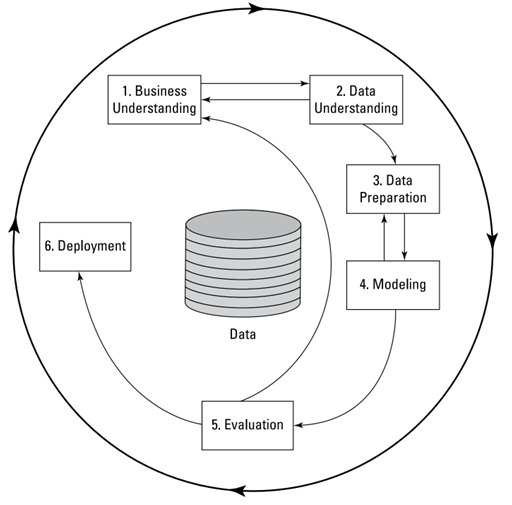
\includegraphics[height=150pt]{Assignment/Phase1-5_new/charts/CRISP-DM.png}\\[4pt]
%  {\small\textit{Figure 1: CRISP-DM pipeline diagram}}
%\end{center}

%\medskip\noindent
\subsubsection*{Tools and Hardware}

{\renewcommand{\arraystretch}{0.75}
\begin{center}
\begin{tabular}{ll}
\hline
\textbf{Category} & \textbf{Details} \\
\hline
Language / IDE & Python 3.12.3, VS Code, Jupyter Notebook \\
Key Libraries & pandas 3.0.1, numpy 2.4.2, matplotlib 3.10.8, scipy 1.17.1 \\
               & scikit-learn 1.8.0, xgboost 3.2.0, category-encoders 2.9.0, joblib 1.5.3 \\
Data Source    & \href{https://www.kaggle.com/datasets/austinreese/usa-housing-listings}{Kaggle} (Craigslist scrape, January 2020) \\
Hardware       & 2 vCPU, 2 GB RAM, Ubuntu 24 Server \\
\hline
\end{tabular}
\end{center}}%

%\medskip\noindent
\subsubsection*{Complete Project Timeline}

{\renewcommand{\arraystretch}{0.75}
\begin{tabular}{lp{6.5cm}ll}
\hline
\textbf{Task} & \textbf{Description} & \textbf{Start} & \textbf{End} \\
\hline
1.1 & Determine Business Objectives  & 1 May 2026 & 9 May 2026  \\
1.2 & Assess the Situation           & 1 May 2026 & 9 May 2026  \\
1.3 & Determine Data-Mining Goals    & 1 May 2026 & 9 May 2026  \\
1.4 & Produce a Project Plan         & 1 May 2026 & 9 May 2026  \\
\hline
2.1 & Gather Data                    & 9 May 2026  & 23 May 2026 \\
2.2 & Describe Data                  & 9 May 2026  & 23 May 2026 \\
2.3 & Explore Data                   & 9 May 2026  & 23 May 2026 \\
2.4 & Verify Data Quality            & 9 May 2026  & 23 May 2026 \\
\hline
3.1 & Select Data                    & 23 May 2026 & 6 Jun 2026  \\
3.2 & Clean Data                     & 23 May 2026 & 6 Jun 2026  \\
3.3 & Construct Data                 & 23 May 2026 & 6 Jun 2026  \\
3.4 & Integrate Data                 & 23 May 2026 & 6 Jun 2026  \\
3.5 & Format Data                    & 23 May 2026 & 6 Jun 2026  \\
\hline
    & Midterm Presentation           & —           & 13 Jun 2026 \\
\hline
4.1 & Select Modeling Technique      & 6 Jun 2026  & 20 Jun 2026 \\
4.2 & Generate Test Design           & 6 Jun 2026  & 20 Jun 2026 \\
4.3 & Build Model                    & 6 Jun 2026  & 20 Jun 2026 \\
4.4 & Assess Model                   & 6 Jun 2026  & 20 Jun 2026 \\
\hline
5.1 & Evaluate Results               & 20 Jun 2026 & 4 Jul 2026  \\
5.2 & Review Process                 & 20 Jun 2026 & 4 Jul 2026  \\
5.3 & Determine Next Steps           & 20 Jun 2026 & 4 Jul 2026  \\
\hline
6.1 & Plan Deployment                & 4 Jul 2026  & 11 Jul 2026 \\
6.2 & Plan Monitoring                & 4 Jul 2026  & 11 Jul 2026 \\
6.3 & Final Report and Presentation  & 4 Jul 2026  & 1 Aug 2026  \\
6.4 & Review Project                 & 4 Jul 2026  & 1 Aug 2026  \\
\hline
\end{tabular}
}%
